\documentclass[10pt,twocolumn,letterpaper]{article}

\usepackage{cvpr}
\usepackage{times}
\usepackage{epsfig}
\usepackage{graphicx}
\usepackage{amsmath}
\usepackage{amssymb}

% Include other packages here, before hyperref.

% If you comment hyperref and then uncomment it, you should delete
% egpaper.aux before re-running latex.  (Or just hit 'q' on the first latex
% run, let it finish, and you should be clear).
\usepackage[breaklinks=true,bookmarks=false]{hyperref}

\cvprfinalcopy % *** Uncomment this line for the final submission

\def\cvprPaperID{****} % *** Enter the CVPR Paper ID here
\def\httilde{\mbox{\tt\raisebox{-.5ex}{\symbol{126}}}}

% Pages are numbered in submission mode, and unnumbered in camera-ready
%\ifcvprfinal\pagestyle{empty}\fi
\setcounter{page}{1}
\begin{document}

%%%%%%%%% TITLE
\title{Fully Convolutional Networks for Image Segmentation with keras}

\author{Giacomo Barzon\\
{\tt\small giacomo.barzon.2@studenti.unipd.it}
% For a paper whose authors are all at the same institution,
% omit the following lines up until the closing ``}''.
% Additional authors and addresses can be added with ``\and'',
% just like the second author.
% To save space, use either the email address or home page, not both
\and
Giacomo Greggio\\
{\tt\small giacomo.greggio.1@studenti.unipd.it}
\and
Diego Mazzalovo\\
{\tt\small diego.mazzalovo@studenti.unipd.it}
}
\maketitle
%\thispagestyle{empty}

%%%%%%%%% ABSTRACT
\begin{abstract}
	"Fully Convolutional Networks for Semantic Segmentation"\cite{projectPaper} is one of the most important piece of work related to Image Semantic Segmentation. Image segmentation is the process of partitioning a digital image into multiple segments (sets of pixels).
	More precisely, image segmentation is the process of assigning a label to every pixel in an image such that pixels with the same label share certain characteristics\cite{wiki}. \\
	Our aim is to reproduce the architectures proposed by the authors which are based on Fully Convolutional Networks (FCNs) with skip connections.
	We trained these architectures on the SBD dataset \cite{dataset}, then we tested it on the PASCAL 2011 validation set. Since some images are both in SBD and in PASCAL VOC 2011 validation set, we tested only on the non-intersecting set between them. The maximum meanIU that we have been able to achieve is 0.57.
\end{abstract}

%%%%%%%%% BODY TEXT
\section{Introduction}

When we talk about Image data there are many tasks that can come to mind. The easiest one that someone can implement is image classification: you give as input an image to the suitable classifier and this one returns the label related to the object that it represents. \\
This approach to image classification has some serious limits, for example if your image contains various objects belonging to several different classes, it's basically impossible to find the correct label since multiple labels will be associated to that image. Moreover in many applications knowing the content of an image is not enough, and it comes necessary to find the locations of the objects depicted in it. \\
The next step to naive image classification is object detection. In object detection, we not only need to identify all the objects of interest in the image, but also their positions. The positions are generally represented by a rectangular bounding box. \\
This approach can be improved because the boxes don't identify perfectly the object boundaries. In many fields like autonomous driving or medical applications knowing the exact boundaries of the objects that we want to identify is essential.
So, the next step that can be made to improve object detection is image segmentation.
Image segmentation is the task of clustering parts of an image together which belong to the same object class. The predictions are made over each pixel which is classified according to a category which can be background or the class it is associated to. \\
There are many more tasks related to image data, but we will focus only on image segmentation. \\ \\
Image classification task are often handled by convolutional networks that have fully connected dense layers at the end of the network. This approach may be fine for many different applications but can pose some serious limitations for image segmentation. The main one is that dense layers unlike convolutional ones can't handle images of various size. To solve this problem many different approaches have been proposed like resizing the images or patch sampling. Those will be discuss better in the next section. \\ \\
All of these methods though can handle only fixed input size or require complicated preprocessing and machinery in order to work. In fully convolutional networks (FCNs) dense layers are substituted by convolutional ones, to make them capable to manage images of any size and produce an output of the same size of the image.


\section{Related Work}

There are many different approaches to solve semantic segmentation problems. The most common approach involves ConvNets with dense predictions. Since they can't handle input of different sizes, many different preprocessing techniques had to be taken in order to make segmentation work. For example, by sampling an area of fixed dimension around each pixel and  using that to classify the pixel. Some previous works have been done by Ning et al.\cite{1495508}, Cirean et al.\cite{article}, where they applied image segmentation respectively to the evolution of embryos and to neuroanatomy. \\
This method computes a prediction pixel by pixel, so both training and predicting, are computationally not efficient. \\ \\
As time passed better approaches have been developed like FCNs that we will discuss in the other chapters, but also many other different techniques.\\
For example one of the most popular ways (from what we have seen) to solve semantic segmentation is through the use of encoder-decoder architectures (see fig. \ref{ednet}).
\begin{figure}[t]
	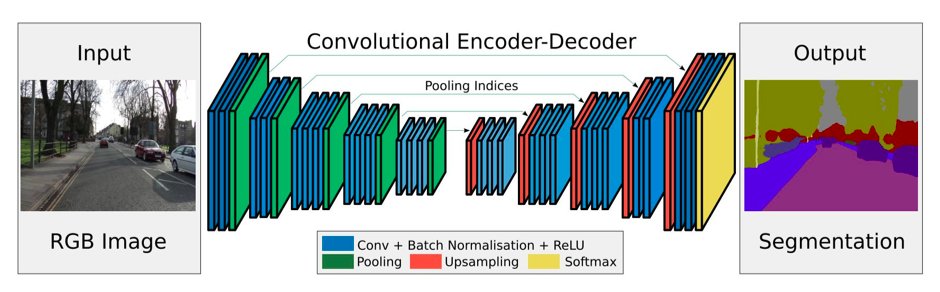
\includegraphics[width=8cm]{image/ednet}
	\label{ednet}
	\centering
	\caption{Encoder-decoder architecure}
\end{figure}
The encoder-decoder architecures are made by two parts: an encoder using convolutional layers (usually taken by VGG16) and a deconvolutional network which takes in input the feature vector produced by the encoder and generates a map of pixelwise class probabilities. Some works have been made by Li et al.\cite{8379359} and Weng et al.\cite{8681706}.\\ \\
Many different approaches based on recursive and recurrent neaural networks have also been proposed, but we didn't dive to much on that. For a more detailed description of the state of the art check the survey made by Minaee et al.\cite{unknown}. 


\section{Dataset}
\subsection{Description}
Since our goal is to reproduce one or more experiments made by the reference paper\cite{projectPaper}, we chose to use the PASCAL VOC 2011\cite{pascal-voc-2011} dataset in which the authors tested all their architectures.
The dataset refers to a visual object challenge made in 2011 and which has been updated in the next years. \\
The dataset contains more than 10000 images with annotations related to different tasks like classification, object detection and image segmentation.
For our task it contains 2223 images, which are 1112 for training set and 1111 for validation set.
The segmentation data is composed by 21 different classes, including background, and a void label which is used to identify the pixels that are ambiguous or difficult to classify, these pixel should be ignored when calculating the loss value. \\ \\
In order to obtain better results, the authors of the paper decided to use a bigger dataset, the SBD dataset \cite{dataset}, which includes 8498 train images, while still keeping the validation set of PASCAL VOC 2011. Some of the images in PASCAL VOC 2011 validation set  are included in SBD dataset. So, to avoid unfair model testing, we removed from the validation set those images that are included in both sets. The authors of this paper take this techniques from "Semantic Boundaries Dataset and Benchmark"\cite{BharathICCV2011}. \\
In the end as validation data we used a subset of 736 images.  \\ \\
\subsection{Preprocessing}
All the segmentation datasets contain two main components: the image data and the mask data. Image data do not require more explanations. Mask data are the classification targets, they have the same shape of the images related to them and each pixel in the mask represent the class it belongs to.
\\ \\
All the datasets needed a minimum amount of preprocessing.
Since all the mask are in RGB format and the neural network returns a probability distribution over each class, we needed to convert the three channels to a single channel representing in each entry the corresponding class. Initially we converted each image to a one-hot-encoding where the number of channels was equal to the number of classes. After some experiments we found out that this wasn't necessary, so we decided to use a lighter version with only one channel. \\

Since we couldn't load the entire dataset in the memories of our PCs, we were forced to build a data generator. A data generator is an object which can be called by keras and returns only the data required to execute a single batch step. This allowed us to keep in memory much less data.

\section{Method}

The authors of \cite{projectPaper} wrote all of their implementations using Caffe \footnote{\href{https://caffe.berkeleyvision.org/}{Link to Caffe}}, a public library with many tools suitable for computer vision. On the other hand we used for all our implementations Keras \footnote{\href{https://keras.io/}{Link to Keras}} library. \\
One of the first things we did was reproducing the architectures that were illustrated in the paper. The most basic architecture between the ones that we reproduced is the FCN32. This architecture is made starting from the VGG16 architecture \cite{weights}.
\begin{figure}[t]
	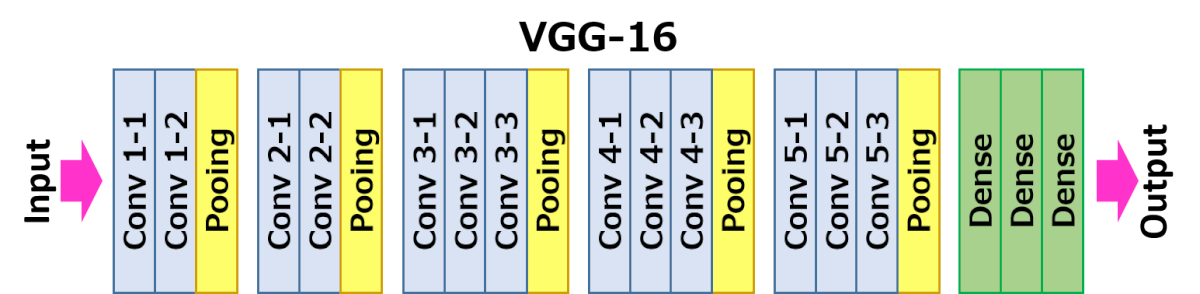
\includegraphics[width=8cm]{image/vgg16}
	\label{vgg}
	\centering
	\caption{VGG16 architecure}
\end{figure}
Like we can see in \ref{vgg} the VGG16 architecture is made by five convolutional blocks, each one contains two or three convolutional layers followed by a MaxPooling layer. After those convolutional blocks there are three fully connected dense layers, which are responsible to make predictions.
\subsection{FCN-32}
We started by replicating the whole VGG16 network with basic keras layers. Since we needed the network to handle inputs of various sizes, we removed the last three fully connected dense layers of the VGG16. Then, we downloaded the pretrained weights of the remaining layers of the network available in the public library of keras.
Like the authors of \cite{projectPaper} did, we appended at the end of the networks three convolutional layers. The first one has a number of filters of 4096 and a kernel size of (7x7). The second one also has a number of filters of 4096, but a kernel size of (1x1). The last one has a number of filters equal to the number of classes we want to predict and a kernel size of (1x1).
These last three layers act in substitution of the dense layers that we removed from the original VGG16. They are the ones who make predictions, but since they are convolutional, they can still handle inputs of any size.
Moreover between each one of these last three convolutional layers we also put a dropout layer with p=0.5.\\
As of now the network outputs a tensor which has a size significantly lower than the one of the input image. Since we want the output to have the same size of the input, we needed to add a deconvolutional layer of size (64x64) with stride 32. This layer increases the size of the input it receives by applying a deconvolution operation. In keras this layer takes the name of Conv2DTranspose \footnote{\href{https://www.tensorflow.org/api_docs/python/tf/keras/layers/Conv2DTranspose}{Link to Conv2DTranspose}}. However, this operation made the output of the network too big by a few extra pixels.\\
\begin{figure*}
	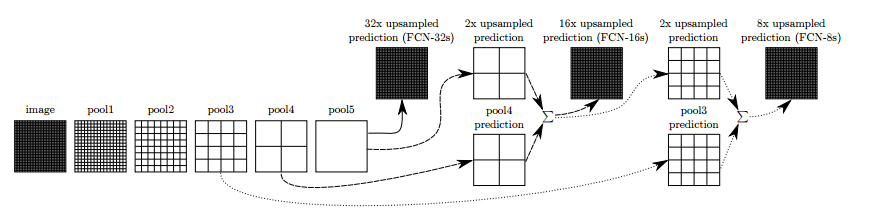
\includegraphics[width=\textwidth]{image/fcn}
	\label{fcn}
	\centering
	\caption{FCN architecure}
\end{figure*}
To solve the problem the authors of the paper added a Cropping layer which takes in input the outputs of two layers and resizes the biggest one to the dimension of the smaller one by removing the extra pixels from the borders. Keras, by default, provides a cropping layer that can crop from images a fixed amount of pixels. This is a serious limitation, since we want to handle images of various sizes. To solve this problem we needed to implement a custom layer which performs the dynamic crop operation as in Caffè. \\ At the end of the network there is a softmax layer in order to produce a valid probability distribution over each class.
\subsection{FCN-16}
FCN-32 architecture is fine, but it can be improved. A way to improve performances is by implementing skip architectures. The receptive fields of the deeper layers are bigger and see more pixels if compared with the shallower ones. This causes FCN32 to produce coarse outputs. Combining the outputs of the deeper layers with the outputs of the shallower ones, allows the model to make more local predictions while respecting the global structure. \\
FCN16 is built on this idea. We take the output of the fourth convolutional block of FCN32 and apply a convolution to it with kernel size of (1x1) and number of filters equal to the number of classes that we want to predict. Then, we sum it with the last convolutional layer of FCN32, the one immediately before the deconvolutional layer. We call this operation fusion  as the original paper. The dimension of the obtained convolutional layer is bigger than the one of the last convolutional layer, due to an higher amount of pooling operations applied to this last layer. 
To make the dimensions of their outputs match we apply to the smaller one a deconvolution with number of filters equal to the number of classes, kernel size of (1x1) and stride equal to 2. We crop the extra pixels with our custom cropping layer like we did at the end of FCN32. Then to make the dimensions of the output match the input dimensions we applied another time a deconvolution followed by a crop.
\subsection{FCN-8}
FCN16 improves a lot the results of FCN32, but it can still be improved. To do that, we follow the same process we used to build FCN16 with some small differences and obtain FCN8.
We take the output of the third convolutional block of VGG16 and apply a convolution to it with the same parameters as the previous architecture and fuse it with the fusion layer of FCN16. As we have done with FCN16 we applied a deconvolution with kernel size of (4x4), stride equal to 2 and number of filters equal to the number of classes. We need to crop the biggest layer between the two before fusing them together. As last layer we make the convolution of the fusion layer with number of filters equal to the number of classes, kernel size of (16x16) and stride equal to 8 which has to be cropped in order to obtain the same dimensions as the input image. The last layer is a softmax layer that produces a valid probability distribution over each class. \\
On all convolutional layers we applied padding in order to obtain the same dimension of the input images. Moreover, all convolutional layers had ReLU as activation function, while the others had a linear activation function. \\ \\
Like the authors of \cite{projectPaper} we didn't bother fusing even shallowers layers, since also between FCN-16 and FCN-8, they got just a small improvement.


\section{Experiments}
\subsection{Normalization}
In order to avoid the gradient explosion we normalized the images in order to obtain pixel values between 0 and 1. In the beginning we made this process by dividing each pixel of the image by the maximum obtainable value of 255. After many tests we noticed that this approach to normalization made the net not converge. \\
So, we implemented the normalization as in the paper by subtracting from each channel the mean of that channel value, averaged on all training images.
\subsection{Optimizer}
The authors of original paper used standard SGD as optimizer. We tried to train our model also with Adam optimizer, but it didn't bring better results. We noticed a faster convergence on the training set, but a worse generalization error.
\subsection{Learning rate}
We tried different learning rates.
We also tried to reduce the learning rate when the training didn't improve performances after a predefined number of epochs, but this didn't improve the results.
In the end the model that obtain the best performances had a fixed learning rate of $ 10^{-4}$ as in the original paper. \\
Moreover they used a doubled learning rate for the biases. Since Keras doesn't let us do it in an easy way, we decided to not spend time to implement it since we don't think it would improve the convergence significately.
\begin{figure*}
	\centering
	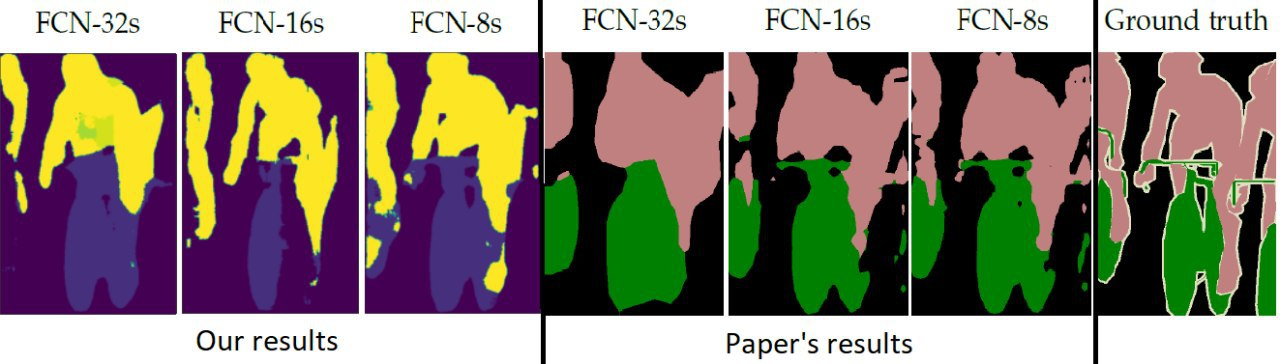
\includegraphics[width=\textwidth]{image/res}
	\caption{Images results comparison}
	\label{fig:results}
\end{figure*}
\subsection{Batch size and momentum}
The authors, in the original paper, train their models with either batch size of 20 and momentum 0.9 or batch size of 1 and momentum 0.99.
We tried many different combinations of those hyperparameters, but in the end we noticed that batch size of 1 and momentum of 0.99 brought the best results.
\subsection{Dropout}
We used the same dropout layers of the original paper, but we noticed that the network converged to similar results even without them.
\subsection{Images with fixed dimensions}
From what we understood the authors of the original paper trained their network with images resized to a fixed size. To do that they resize each image to the dimensions of the biggest image in the dataset, by adding extra ignorable pixels to the edges. \\
To use batch size greater than 1 with images of varying size, all samples in the batch need to have the same dimension. In the beginning we resized all images to a fixed size. After seeing that we got the best performances with batch size equal to 1, we decided to use the original not resized images with variable size, since they use less space. \\
Moreover we also noticed that with the resized images the network spent a lot of time in learning the pattern proceduced by the resizing instead of learning how to recognize the objects.
\subsection{Regularization}
The authors of the paper added weight decay regularization to the loss with values of $ 5^{-4}$ and $ 2^{-5}$ for the different nets. Unfortunately Keras doesn't allow to add a global regularization effect like Caffè, so we tried to replicate it by adding it manually to each layer, but the regularization always led the networks to not converge no matter its value.
In the end, we achieved the best results with a net without any kind of regularization.
\subsection{Initialization}
The authors of the original paper initialized the weights of the scoring layers (all the convolutional layers with the number of filters equal to the number of classes) with a zero initialization. Since this didn't influence much the results we decided to omit it. \\ \\
The authors also initialized the weights of deconvolutional layers to the bilinear interpolation. Unfortunately Keras doesn't offer this kind of initialization, so we didn't spend time to create our custom initializer, since we don't think it would have improved the results.

\section{Conclusions}
\begin{table}[htp]
	\begin{center}
		\begin{tabular}{|c|c|c|}
			\hline
			Architecture & Our MeanIU & Paper's MeanIU\\
			\hline\hline
			FCN32 & 0.565 & 0.636\\
			FCN16 & 0.570 & 0.650\\
			FCN8 & 0.533 & 0.655\\
			\hline
		\end{tabular}
	\end{center}
	\caption{MeanIU results comparison}
	\label{mytable}
\end{table}
The results we obtained are decent, but still far from the results obtained in the original paper. The network which performed better has been FCN16 which reached a MeanIU of 0.570. The improvement that we obtained with FCN16 is really small, but also in the original paper they didn't obtain a big improvement on this dataset. \\
On the other hand, FCN8 got worse results than the previous two architectures. FCN8 is a complex network and the training probably suffered a lot from the absence of the regularization. Despite our many attempts to make it work we always obtained worse results when we applied regularization to our architecture. \\
Despite the worse MeanIU, FCN8 seems to learn better the shapes of the objetcs, but it often classifies wrongly the pixels, as we can see from fig. \ref{fig:results} .
We didn't try to replicate all of the experiments that were made in the paper, for example:
\begin{itemize}
	\item training and testing the architectures on different datasets like PASCAL Context, Sift Flow, Nyuv V2.
	\item training other architectures like GoogleNet and AlexNet.
	\item training by giving masked out input images.
	\item staged training.
\end{itemize}


{\small
\bibliographystyle{ieee_fullname}
\bibliography{egbib}
}

\end{document}
